\documentclass[]{article}
\usepackage{lmodern}
\usepackage{amssymb,amsmath}
\usepackage{ifxetex,ifluatex}
\usepackage{fixltx2e} % provides \textsubscript
\ifnum 0\ifxetex 1\fi\ifluatex 1\fi=0 % if pdftex
  \usepackage[T1]{fontenc}
  \usepackage[utf8]{inputenc}
\else % if luatex or xelatex
  \ifxetex
    \usepackage{mathspec}
  \else
    \usepackage{fontspec}
  \fi
  \defaultfontfeatures{Ligatures=TeX,Scale=MatchLowercase}
\fi
% use upquote if available, for straight quotes in verbatim environments
\IfFileExists{upquote.sty}{\usepackage{upquote}}{}
% use microtype if available
\IfFileExists{microtype.sty}{%
\usepackage{microtype}
\UseMicrotypeSet[protrusion]{basicmath} % disable protrusion for tt fonts
}{}
\usepackage[margin=1in]{geometry}
\usepackage{hyperref}
\hypersetup{unicode=true,
            pdftitle={Estimation Methods of ABO-Gene Allele Frequency in Population using Phenotypic Blood-Type Data. Estimating ABO-Gene Allele Frequency in Population using Phenotypic Blood-Type Data.},
            pdfauthor={Faizan Khalid Mohsin},
            pdfborder={0 0 0},
            breaklinks=true}
\urlstyle{same}  % don't use monospace font for urls
\usepackage{color}
\usepackage{fancyvrb}
\newcommand{\VerbBar}{|}
\newcommand{\VERB}{\Verb[commandchars=\\\{\}]}
\DefineVerbatimEnvironment{Highlighting}{Verbatim}{commandchars=\\\{\}}
% Add ',fontsize=\small' for more characters per line
\usepackage{framed}
\definecolor{shadecolor}{RGB}{248,248,248}
\newenvironment{Shaded}{\begin{snugshade}}{\end{snugshade}}
\newcommand{\KeywordTok}[1]{\textcolor[rgb]{0.13,0.29,0.53}{\textbf{#1}}}
\newcommand{\DataTypeTok}[1]{\textcolor[rgb]{0.13,0.29,0.53}{#1}}
\newcommand{\DecValTok}[1]{\textcolor[rgb]{0.00,0.00,0.81}{#1}}
\newcommand{\BaseNTok}[1]{\textcolor[rgb]{0.00,0.00,0.81}{#1}}
\newcommand{\FloatTok}[1]{\textcolor[rgb]{0.00,0.00,0.81}{#1}}
\newcommand{\ConstantTok}[1]{\textcolor[rgb]{0.00,0.00,0.00}{#1}}
\newcommand{\CharTok}[1]{\textcolor[rgb]{0.31,0.60,0.02}{#1}}
\newcommand{\SpecialCharTok}[1]{\textcolor[rgb]{0.00,0.00,0.00}{#1}}
\newcommand{\StringTok}[1]{\textcolor[rgb]{0.31,0.60,0.02}{#1}}
\newcommand{\VerbatimStringTok}[1]{\textcolor[rgb]{0.31,0.60,0.02}{#1}}
\newcommand{\SpecialStringTok}[1]{\textcolor[rgb]{0.31,0.60,0.02}{#1}}
\newcommand{\ImportTok}[1]{#1}
\newcommand{\CommentTok}[1]{\textcolor[rgb]{0.56,0.35,0.01}{\textit{#1}}}
\newcommand{\DocumentationTok}[1]{\textcolor[rgb]{0.56,0.35,0.01}{\textbf{\textit{#1}}}}
\newcommand{\AnnotationTok}[1]{\textcolor[rgb]{0.56,0.35,0.01}{\textbf{\textit{#1}}}}
\newcommand{\CommentVarTok}[1]{\textcolor[rgb]{0.56,0.35,0.01}{\textbf{\textit{#1}}}}
\newcommand{\OtherTok}[1]{\textcolor[rgb]{0.56,0.35,0.01}{#1}}
\newcommand{\FunctionTok}[1]{\textcolor[rgb]{0.00,0.00,0.00}{#1}}
\newcommand{\VariableTok}[1]{\textcolor[rgb]{0.00,0.00,0.00}{#1}}
\newcommand{\ControlFlowTok}[1]{\textcolor[rgb]{0.13,0.29,0.53}{\textbf{#1}}}
\newcommand{\OperatorTok}[1]{\textcolor[rgb]{0.81,0.36,0.00}{\textbf{#1}}}
\newcommand{\BuiltInTok}[1]{#1}
\newcommand{\ExtensionTok}[1]{#1}
\newcommand{\PreprocessorTok}[1]{\textcolor[rgb]{0.56,0.35,0.01}{\textit{#1}}}
\newcommand{\AttributeTok}[1]{\textcolor[rgb]{0.77,0.63,0.00}{#1}}
\newcommand{\RegionMarkerTok}[1]{#1}
\newcommand{\InformationTok}[1]{\textcolor[rgb]{0.56,0.35,0.01}{\textbf{\textit{#1}}}}
\newcommand{\WarningTok}[1]{\textcolor[rgb]{0.56,0.35,0.01}{\textbf{\textit{#1}}}}
\newcommand{\AlertTok}[1]{\textcolor[rgb]{0.94,0.16,0.16}{#1}}
\newcommand{\ErrorTok}[1]{\textcolor[rgb]{0.64,0.00,0.00}{\textbf{#1}}}
\newcommand{\NormalTok}[1]{#1}
\usepackage{longtable,booktabs}
\usepackage{graphicx,grffile}
\makeatletter
\def\maxwidth{\ifdim\Gin@nat@width>\linewidth\linewidth\else\Gin@nat@width\fi}
\def\maxheight{\ifdim\Gin@nat@height>\textheight\textheight\else\Gin@nat@height\fi}
\makeatother
% Scale images if necessary, so that they will not overflow the page
% margins by default, and it is still possible to overwrite the defaults
% using explicit options in \includegraphics[width, height, ...]{}
\setkeys{Gin}{width=\maxwidth,height=\maxheight,keepaspectratio}
\IfFileExists{parskip.sty}{%
\usepackage{parskip}
}{% else
\setlength{\parindent}{0pt}
\setlength{\parskip}{6pt plus 2pt minus 1pt}
}
\setlength{\emergencystretch}{3em}  % prevent overfull lines
\providecommand{\tightlist}{%
  \setlength{\itemsep}{0pt}\setlength{\parskip}{0pt}}
\setcounter{secnumdepth}{0}
% Redefines (sub)paragraphs to behave more like sections
\ifx\paragraph\undefined\else
\let\oldparagraph\paragraph
\renewcommand{\paragraph}[1]{\oldparagraph{#1}\mbox{}}
\fi
\ifx\subparagraph\undefined\else
\let\oldsubparagraph\subparagraph
\renewcommand{\subparagraph}[1]{\oldsubparagraph{#1}\mbox{}}
\fi

%%% Use protect on footnotes to avoid problems with footnotes in titles
\let\rmarkdownfootnote\footnote%
\def\footnote{\protect\rmarkdownfootnote}

%%% Change title format to be more compact
\usepackage{titling}

% Create subtitle command for use in maketitle
\providecommand{\subtitle}[1]{
  \posttitle{
    \begin{center}\large#1\end{center}
    }
}

\setlength{\droptitle}{-2em}

  \title{Estimation Methods of ABO-Gene Allele Frequency in Population using
Phenotypic Blood-Type Data. Estimating ABO-Gene Allele Frequency in
Population using Phenotypic Blood-Type Data.}
    \pretitle{\vspace{\droptitle}\centering\huge}
  \posttitle{\par}
    \author{Faizan Khalid Mohsin}
    \preauthor{\centering\large\emph}
  \postauthor{\par}
      \predate{\centering\large\emph}
  \postdate{\par}
    \date{September 22, 2020}


\begin{document}
\maketitle

\section{Introduction}\label{introduction}

We have a theoretical frame work where we know that pairing combinations
of the 3 alleles (antigens: A, B, O) on the ABO-gene (ABO locus) found
on chromosome 9, lead to four phenotypic manifestations in the form of 4
blood types: A, B, AB, O.

Now, there is an interest in estimating the frequency of the 3 alleles
A, B, O in the population. One way to do this would be to take blood
samples of a big sample of people from the population of interest and
using DNA sequencing to determine the allele type (A or B or O) on the
ABO-gene on chromosome 9. However, to get reliable frequency estimates
one needs to do to DNA sequency for a large number of people, which will
be extremely expensive and time consuming. A more practical and more
efficient method for estimating the 3 allele frequencies of a population
would be to collect the phenotypic data, the blood type A, B, AB or O of
people, which would be much more cheaper and easier to do at a large
scale and using the theoretical framework to estimate the 3 allele
frequencies in the population using the phenotypic blood type data.

In this paper we will layout the theoretical framework for estimating
the allele frequency using phenotypic blood type data and use two
separate algorithms and approaches for the estimation. Finally, we will
use the actual blood type data gathered from a sample of 2114 people to
demonstrate and estimate the allele frequency using the two algorithms.

\section{Method}\label{method}

We use two methods for approximating the allele frequencies:
Expectation-Maximization method and Newton-Raphson method.

In the ideal case we could sample n people and find out how many people
possess allele A (nA), how many possess allele B (nB) and how many
possess allele (nO). In such a case it would be very easy to calculate
the allele frequency in the population: freq(A) = nA/n, freq(B) = nB/n,
and freq(O) = nO/n. And we would be done. However, getting nA, nB, nO
directly from DNA sequencing is very expensive and time consuming. It is
much easier to collect the blood type of each individual from the sample
of n people. This will give us a numeric count of how many people have
each blood type, namely, n\_A: number of people with blood type A, n\_B:
number of people with blood type B, n\_AB: number of people with blood
type AB and n\_O: number of people with blood type O. We use genetics to
link the number of individuals with alleles nA, nB, and nO with number
of people with phenotypes n\_A, n\_B, n\_AB, and n\_O (blood-type).

\subsection{Theoretical Framework.}\label{theoretical-framework.}

\subsubsection{Genetical Theory}\label{genetical-theory}

From genetic theory we know that alleles A, B are dominant to allele O;
alleles A, B are co-dominant; and allele O is recessive to alleles A, B.
Using this below is a mapping from genotype to phenotype. Genotype
Phenotype AA or AO - A BB or BO - B AB - AB OO - O

\subsubsection{Hardy--Weinberg
equilibrium.}\label{hardyweinberg-equilibrium.}

\[p=freq(\mbox{allele } A),\] \[q=freq(\mbox{allele } B),\]
\[1-p-q=freq(\mbox{allele } O).\]

\[freq(AA)=p^2, \: \:  freq(AO)=2p(1-p-q),\]
\[freq(BB)=q^2, \: \: freq(BO)=2q(1-p-q),\]
\[freq(AB)=2pq, \: \: freq(OO)=(1-p-q)^2.\]

\[freq(A)=p^2+2p(1-p-q),\] \[freq(B)=q^2+2q(1-p-q),\] \[freq(AB)=2pq,\]
\[freq(O)=(1-p-q)^2.\]

Going from allele frequency to genotypic frequency and going from
genotypic frequency to phenotypic frequency.

he Hardy-Weinberg principle states that a population's allele and
genotype frequencies will remain constant in the absence of evolutionary
mechanisms. Ultimately, the Hardy-Weinberg principle models a population
without evolution under the following conditions:

no mutations no immigration/emigration no natural selection no sexual
selection a large population Although no real-world population can
satisfy all of these conditions, the principle still offers a useful
model for population analysis.

Hardy-Weinberg Equations and Analysis According to the Hardy-Weinberg
principle, the variable p often represents the frequency of a particular
allele, usually a dominant one. If p and q are the only two possible
alleles for this characteristic, then the sum of the frequencies must
add up to 1, or 100 percent. We can also write this as p + q = 1. If the
frequency of the Y allele in the population is 0.6, then we know that
the frequency of the y allele is 0.4.

From the Hardy-Weinberg principle and the known allele frequencies, we
can also infer the frequencies of the genotypes. Since each individual
carries two alleles per gene (Y or y), we can predict the frequencies of
these genotypes with a chi square. If two alleles are drawn at random
from the gene pool, we can determine the probability of each genotype.

The Hardy-Weinberg principle assumes that in a given population, the
population is large and is not experiencing mutation, migration, natural
selection, or sexual selection. The frequency of alleles in a population
can be represented by p + q = 1, with p equal to the frequency of the
dominant allele and q equal to the frequency of the recessive allele.
The frequency of genotypes in a population can be represented by
p2+2pq+q2= 1, with p2 equal to the frequency of the homozygous dominant
genotype, 2pq equal to the frequency of the heterozygous genotype, and
q2 equal to the frequency of the recessive genotype. The frequency of
alleles can be estimated by calculating the frequency of the recessive
genotype, then calculating the square root of that frequency in order to
determine the frequency of the recessive allele.

How reasonable is it to assume HWE.

\subsubsection{Statistical Theory:}\label{statistical-theory}

We have our log likelihood function:

\[ln(L) \sim n_\text{A}\ln\left(p^2+2\left(-p q+1\right)p\right)+n_\text{AB}\ln\left(2qp\right)+2n_\text{O}\ln\left(-p-q+1\right)+n_\text{B}\ln\left(2q\left(-p-q+1\right)+q^2\right)
\]

We can find the maxima's of this by taking the first derivative,
equating to zero and then solving for p and q. However, this is very
difficult to do analytically. Hence, we will use two different
algorithms and approaches to estimate p and q. Namely, the
Estimation-Maximization algorithm and the Newton-Raphson algorithm.

\subsection{Newton-Raphson Algorithm
Method}\label{newton-raphson-algorithm-method}

The other method is a more direct method where we directly find the
maxima's of the loglikelihood function using numeric computational
method called Newton-Raphson algorithm.

To approximate the values of \(\hat{p}, \hat{q}.\)

Using the properties of log we can be simplified to the following:

\[ln(L) \sim n_\text{B}\ln\left(-q\left(2p+q-2\right)\right)+n_\text{A}\ln\left(-p\left(p+2q-2\right)\right)+n_\text{AB}\ln\left(2qp\right)+2n_\text{O}\ln\left(-p-q+1\right)
\]

We need to get the full first derivative of this with respect to p and
q.

\item 

A numerical iterative approach to obtain the maximum (or the minimum) a
function: \(f(\vec \theta)\), \((\vec \theta \in R^n)\), e.g.
\[f(\vec \theta) = lnL(p,q) = f(p,q)\] \smallskip

\item 

It is based on the first derivatives (gradient vector),
e.g.\textbackslash{}

\[ f'(\vec \theta) = f'(p,q) = 
\left[ \begin{array}{c} 
\frac{\partial{f(p,q)}}{\partial{p}}\\
\frac{\partial{f(p,q)}}{\partial{q}}
\end{array} \right] \] \bigskip

and the second derivatives (Hessian matrix), e.g.\textbackslash{}

\[ f''(\vec \theta) = f''(p,q) = 
\left[ \begin{array}{cc} 
\frac{\partial^2 {f(p,q)}}{{\partial{p}}^2}&
\frac{\partial^2 {f(p,q)}}{\partial{p}\partial{q}}\\
\frac{\partial^2 {f(p,q)}}{\partial{q}\partial{p}}&
\frac{\partial^2 {f(p,q)}}{{\partial{q}}^2}
\end{array} \right] \] \bigskip

\item 

The algorithm is such:

\begin{itemize}

\item Choose a starting value, $\vec \theta ^{(0)}$. 

\item For $k=1,2,...$ the updating function is

$$\vec \theta^{(k)} = \vec \theta^{(k-1)} 
- [f''(\vec \theta^{(k-1)})]^{-1} f'(\vec \theta^{(k-1)})$$  
\bigskip

\item Under certain conditions, $\{\vec \theta^{(k)}\}$ converges to the value that maximizes (or minimizes) the function. 
\end{itemize}

\pagebreak

\item 

A few notes on the Newton-Raphson algorithm. \textbackslash{}

\textbackslash{}begin\{itemize\}

\item 

The staring value, \(\vec \theta ^{(0)}\), is important: the algorithm
is not guaranteed to converge from all starting values, particularly in
regions where the matrix \(- [f''(\vec \theta^{(k-1)})]\) is no positive
definite. \textbackslash{}

(Staring values may be obtained from some crude parameter estimates.)
\smallskip

\item 

The advantage of Newton's method is: once the iterates are close to the
solution, convergence is extremely fast. \smallskip

\item 

If the iterations do not converge: they typically move off quickly
toward the edge of the parameter space. \textbackslash{}

(The remedy can be trying again with a new staring point.) \smallskip

\item 

The computational load can be heavy, if the number of parameters is
large, because of the inverse of the Hessian matrix.

We find that the derivative with respect to p is \(df/dp\):

\[ \frac{\partial f}{\partial p } = \dfrac{2n_\text{B}}{2p+q-2}+n_\text{A}\left(\dfrac{1}{p+2q-2}+\dfrac{1}{p}\right)+\dfrac{n_\text{AB}}{p}-\dfrac{2n_\text{O}}{-p-q+1}
\]

The first derivative with respect to q is \(df/dq\):

\[\frac{\partial f}{\partial q } = \dfrac{2n_\text{A}}{2q+p-2}+n_\text{B}\left(\dfrac{1}{q+2p-2}+\dfrac{1}{q}\right)+\dfrac{n_\text{AB}}{q}-\dfrac{2n_\text{O}}{-q-p+1}
\]

The second derivatives which are the components of the hessian are as
follows:

\(d^2f/dp^2\)

\[ \frac{\partial^2 f}{\partial p^2} = -\dfrac{4n_\text{B}}{\left(2p+q-2\right)^2}+n_\text{A}\left(-\dfrac{1}{\left(p+2q-2\right)^2}-\dfrac{1}{p^2}\right)-\dfrac{n_\text{AB}}{p^2}-\dfrac{2n_\text{O}}{\left(-p-q+1\right)^2}
\]

\(d^2f/dqdp\)

\[\frac{\partial^2 f}{\partial q \partial p } = -\dfrac{2n_\text{B}}{\left(2p+q-2\right)^2}-\dfrac{2n_\text{A}}{\left(p+2q-2\right)^2}-\dfrac{2n_\text{O}}{\left(-p-q+1\right)^2}
\]

\(d^2f/dq^2\)

\[ \frac{\partial^2 f}{\partial q^2} = -\dfrac{4n_\text{A}}{\left(2q+p-2\right)^2}+n_\text{B}\left(-\dfrac{1}{\left(q+2p-2\right)^2}-\dfrac{1}{q^2}\right)-\dfrac{n_\text{AB}}{q^2}-\dfrac{2n_\text{O}}{\left(-q-p+1\right)^2}
\]

\(d^2f/dpdq\)

\[\frac{\partial^2 f}{\partial p \partial q } =-\dfrac{2n_\text{B}}{\left(2p+q-2\right)^2}-\dfrac{2n_\text{A}}{\left(p+2q-2\right)^2}-\dfrac{2n_\text{O}}{\left(-p-q+1\right)^2}
\]

\subsection{Estimation-Maximization Algorithm
Method}\label{estimation-maximization-algorithm-method}

One method to solving this is to think of the allele frequencies as
latent variables or missing variables. In this approach we can cast the
problem in the framework of EM algorithm.

To implement the EM algorithm we reframe the question in terms of a
missing data problem.

\item 

The Expectation-Maximization (EM) algorithm is a numerical iterative
method for finding the Maximum Likelihood Estimates (MLE) of parameters.
\smallskip

\item 

EM algorithms are often used in situations where the problem of
estimation can be solved much easier if certain additional pieces of
data are available. \pagebreak

\item 

The ABO-blood problem can be formulated as such incomplete data or
missing data problem:

\begin{itemize}

\item Some of the  counts of the 6 genotypes are missing:\\
among blood type A: $n_{A}=n_{AA}+n_{AO}$,\\
among blood type B: $n_{B}=n_{BB}+n_{BO}$.
\smallskip

\item Complete data:\\
$n_{AA}$, $n_{AO}$, $n_{BB}$, $n_{BO}$, $n_{AB}$, $n_{OO}$.
\smallskip

\item Observed data:\\
$n_A=n_{AA}+n_{AO}$, $n_B=n_{BB}+n_{BO}$,
$n_{AB}=n_{AB}$, $n_{O}=n_{OO}$.
\smallskip

\item Missing data:\\
$n_{AA}$ or $n_{AO}$, $n_{BB}$ or $n_{BO}$.
\end{itemize}

\bigskip

\item 

Parameters of interest: \(p=freq(\mbox{allele } A)\) and
\(q=freq(\mbox{allele } B)\). \pagebreak

\item 

E-step: the expected value of the log likelihood is calculated (when the
log likelihood is linear w.r.t. to the missing data as in this case,
then essentially, the missing data are imputed), assuming some initial
values for the parameters, e.g.~given the initial parameter values
\(p^{(0)}\), \(q^{(0)}\):\textbackslash{} \bigskip

\{\small
\$E{[}n\_\{AA\}{]} = \frac{freq(AA)}{freq(AA)+freq(AO)} n\_A
\$\textbackslash{} \hspace*{1.8cm}
\(=\frac{p^{(0)}p^{(0)}}{p^{(0)}p^{(0)}+2p^{(0)}(1-p^{(0)}-q^{(0)})} n_A = n_{AA}^{(0)}\)
\textbackslash{} \bigskip

\(E[n_{AO}] = n_A-n_{AA} = \frac{freq(AO)}{freq(AA)+freq(AO)} n_A\)\textbackslash{}
\hspace*{1.8cm}
\(=\frac{2p^{(0)}(1-p^{(0)}-q^{(0)})}{p^{(0)}p^{(0)}+2p^{(0)}(1-p^{(0)}-q^{(0)})} n_A = n_{AO}^{(0)}\)
\textbackslash{} \bigskip
\bigskip

\$E{[}n\_\{BB\}{]} = \frac{freq(BB)}{freq(BB)+freq(BO)} n\_B
\$\textbackslash{} \hspace*{1.8cm}
\(=\frac{q^{(0)}q^{(0)}}{q^{(0)}q^{(0)}+2q^{(0)}(1-p^{(0)}-q^{(0)})} n_B = n_{BB}^{(0)}\)
\textbackslash{} \bigskip

\(E[n_{BO}] = n_B-n_{BB} = \frac{freq(BO)}{freq(BB)+freq(BO)} n_B\)\textbackslash{}
\hspace*{1.8cm}
\(=\frac{2q^{(0)}(1-p^{(0)}-q^{(0)})}{q^{(0)}q^{(0)}+2q^{(0)}(1-p^{(0)}-q^{(0)})} n_B = n_{BO}^{(0)}\)
\textbackslash{} \} \pagebreak

\item 

M-step: MLE can then be calculated based on
\centerline{imputed missing data + observed data = complete data}
\smallskip

e.g.~MLE of the parameters of interest, \(p\) and \(q\), given the
imputed missing data (\(n_{AA}^{(0)}\), \(n_{AO}^{(0)}\),
\(n_{BB}^{(0)}\), \(n_{BO}^{(0)}\)), and the observed data (\(n_{AB}\),
\(n_{OO}\)):

\[p^{(1)} = \frac{2n_{AA}^{(0)}+n_{AO}^{(0)}+n_{AB}}{2n}\]

\[q^{(1)} = \frac{2n_{BB}^{(0)}+n_{BO}^{(0)}+n_{AB}}{2n}\] \bigskip

where \(n=n_{A}+n_{B}+n_{AB}+n_{O}\), the total number of individuals in
the sample.\textbackslash{}

\(p^{(1)}\) and \(q^{(1)}\) are improved estimates of the parameters!
\pagebreak

\item 

Use \(p^{(1)}\) and \(q^{(1)}\) to perform the E-step again, and then
perform the M-step to obtain improved estimates, \(p^{(2)}\) and
\(q^{(2)}\). \smallskip

\item 

Continue until convergence: the changes in parameter estimates
(\(p^{(k)}-p^{(k-1)}\), \(q^{(k)}-q^{(k-1)}\)) are negligible for the
purpose of the study. \bigskip

\item 

A couple of comments on the EM algorithm: \smallskip
\textbackslash{}begin\{itemize\} \item Under regular conditions, the
algorithm converges to a local mode of the posterior density. \smallskip
\item The rate at which the EM algorithm converges depends on the
proportion of missing ``information''.

\subsection{Sample Space of p \& q and initial
values.}\label{sample-space-of-p-q-and-initial-values.}

\begin{Shaded}
\begin{Highlighting}[]
\NormalTok{a1 =}\StringTok{ }\KeywordTok{seq}\NormalTok{(}\FloatTok{0.03}\NormalTok{, }\DecValTok{1}\NormalTok{, .}\DecValTok{15}\NormalTok{)}
\NormalTok{b1 =}\StringTok{ }\KeywordTok{rep}\NormalTok{(a1[}\DecValTok{1}\NormalTok{], }\KeywordTok{length}\NormalTok{(a1))}
\NormalTok{a2 =}\StringTok{ }\KeywordTok{seq}\NormalTok{(a1[}\DecValTok{1}\NormalTok{], .}\DecValTok{8}\NormalTok{, .}\DecValTok{15}\NormalTok{)}
\NormalTok{b2 =}\StringTok{ }\KeywordTok{rep}\NormalTok{(a1[}\DecValTok{2}\NormalTok{], }\KeywordTok{length}\NormalTok{(a2))}
\NormalTok{a3 =}\StringTok{ }\KeywordTok{seq}\NormalTok{(a1[}\DecValTok{1}\NormalTok{], .}\DecValTok{65}\NormalTok{, .}\DecValTok{15}\NormalTok{)}
\NormalTok{b3 =}\StringTok{ }\KeywordTok{rep}\NormalTok{(a1[}\DecValTok{3}\NormalTok{], }\KeywordTok{length}\NormalTok{(a3))}
\NormalTok{a4 =}\StringTok{ }\KeywordTok{seq}\NormalTok{(a1[}\DecValTok{1}\NormalTok{], .}\DecValTok{50}\NormalTok{, .}\DecValTok{15}\NormalTok{)}
\NormalTok{b4 =}\StringTok{ }\KeywordTok{rep}\NormalTok{(a1[}\DecValTok{4}\NormalTok{], }\KeywordTok{length}\NormalTok{(a4))}
\NormalTok{a5 =}\StringTok{ }\KeywordTok{seq}\NormalTok{(a1[}\DecValTok{1}\NormalTok{], .}\DecValTok{35}\NormalTok{, .}\DecValTok{15}\NormalTok{)}
\NormalTok{b5 =}\StringTok{ }\KeywordTok{rep}\NormalTok{(a1[}\DecValTok{5}\NormalTok{], }\KeywordTok{length}\NormalTok{(a5))}
\NormalTok{a6 =}\StringTok{ }\KeywordTok{seq}\NormalTok{(a1[}\DecValTok{1}\NormalTok{], .}\DecValTok{2}\NormalTok{, .}\DecValTok{15}\NormalTok{)}
\NormalTok{b6 =}\StringTok{ }\KeywordTok{rep}\NormalTok{(a1[}\DecValTok{6}\NormalTok{], }\KeywordTok{length}\NormalTok{(a6))}
\NormalTok{a7 =}\StringTok{ }\NormalTok{a1[}\DecValTok{1}\NormalTok{]}
\NormalTok{b7 =}\StringTok{ }\KeywordTok{rep}\NormalTok{(a1[}\DecValTok{7}\NormalTok{], }\KeywordTok{length}\NormalTok{(a7))}


\NormalTok{pi =}\StringTok{ }\KeywordTok{c}\NormalTok{(a1, a2, a3, a4, a5, a6, a7)}
\NormalTok{qi =}\StringTok{ }\KeywordTok{c}\NormalTok{(b1, b2, b3, b4, b5, b6, b7)}

\CommentTok{# a1}
\CommentTok{# b1}
\CommentTok{# a2}
\CommentTok{# b2}
\CommentTok{# a3}
\CommentTok{# b3}
\CommentTok{# a4}
\CommentTok{# b4}
\CommentTok{# a5}
\CommentTok{# b5}
\CommentTok{# a6}
\CommentTok{# b6}
\CommentTok{# a7}
\CommentTok{# b7}

\CommentTok{# pi }
\CommentTok{# qi }


\KeywordTok{library}\NormalTok{(ggplot2)}
\end{Highlighting}
\end{Shaded}

\begin{verbatim}
## Warning: package 'ggplot2' was built under R version 3.6.3
\end{verbatim}

\begin{Shaded}
\begin{Highlighting}[]
\NormalTok{fun1 <-}\StringTok{ }\ControlFlowTok{function}\NormalTok{(q) }\DecValTok{1} \OperatorTok{-}\StringTok{ }\NormalTok{q}
\NormalTok{fun2 <-}\StringTok{ }\ControlFlowTok{function}\NormalTok{(q) }\DecValTok{0}
\NormalTok{fun3 <-}\StringTok{ }\ControlFlowTok{function}\NormalTok{(q) }\DecValTok{0}
\NormalTok{q =}\StringTok{ }\KeywordTok{seq}\NormalTok{(}\DecValTok{0}\NormalTok{,}\DecValTok{1}\NormalTok{, }\DataTypeTok{length.out =} \KeywordTok{length}\NormalTok{(qi))}
\NormalTok{mydf =}\StringTok{ }\KeywordTok{data.frame}\NormalTok{(q, }\DataTypeTok{p=}\KeywordTok{fun1}\NormalTok{(q), }\DataTypeTok{y2=}\KeywordTok{fun2}\NormalTok{(q),}\DataTypeTok{y3=} \KeywordTok{fun3}\NormalTok{(q))}
\NormalTok{mydf <-}\StringTok{  }\KeywordTok{transform}\NormalTok{(mydf, }\DataTypeTok{z =} \KeywordTok{pmax}\NormalTok{(p,}\KeywordTok{pmin}\NormalTok{(y2,y3)))}
\KeywordTok{ggplot}\NormalTok{(mydf, }\KeywordTok{aes}\NormalTok{(}\DataTypeTok{x =}\NormalTok{ q)) }\OperatorTok{+}\StringTok{ }
\StringTok{  }\KeywordTok{geom_line}\NormalTok{(}\KeywordTok{aes}\NormalTok{(}\DataTypeTok{y =}\NormalTok{ p), }\DataTypeTok{colour =} \StringTok{'blue'}\NormalTok{, }\DataTypeTok{size =} \DecValTok{2}\NormalTok{) }\OperatorTok{+}
\StringTok{  }\KeywordTok{geom_line}\NormalTok{(}\KeywordTok{aes}\NormalTok{(}\DataTypeTok{y =}\NormalTok{ y2), }\DataTypeTok{colour =} \StringTok{'green'}\NormalTok{, }\DataTypeTok{size =} \DecValTok{2}\NormalTok{) }\OperatorTok{+}
\StringTok{  }\KeywordTok{geom_line}\NormalTok{(}\KeywordTok{aes}\NormalTok{(}\DataTypeTok{y =}\NormalTok{ y3), }\DataTypeTok{colour =} \StringTok{'red'}\NormalTok{, }\DataTypeTok{size =} \DecValTok{2}\NormalTok{) }\OperatorTok{+}
\StringTok{  }\KeywordTok{geom_ribbon}\NormalTok{(}\KeywordTok{aes}\NormalTok{(}\DataTypeTok{ymin=}\DecValTok{0}\NormalTok{,}\DataTypeTok{ymax =}\NormalTok{ z), }\DataTypeTok{fill =} \StringTok{'gray60'}\NormalTok{) }\OperatorTok{+}\StringTok{ }
\StringTok{  }\KeywordTok{geom_point}\NormalTok{(}\KeywordTok{aes}\NormalTok{(}\DataTypeTok{x =}\NormalTok{ qi, }\DataTypeTok{y =}\NormalTok{ pi)) }\OperatorTok{+}
\StringTok{  }\KeywordTok{geom_text}\NormalTok{(}\DataTypeTok{x=}\NormalTok{.}\DecValTok{75}\NormalTok{, }\DataTypeTok{y=}\NormalTok{.}\DecValTok{75}\NormalTok{, }\DataTypeTok{label=}\StringTok{"Constraints: }\CharTok{\textbackslash{}n}\StringTok{ p + q < 1 }\CharTok{\textbackslash{}n}\StringTok{ p > 0 }\CharTok{\textbackslash{}n}\StringTok{ q > 0"}\NormalTok{)}
\end{Highlighting}
\end{Shaded}

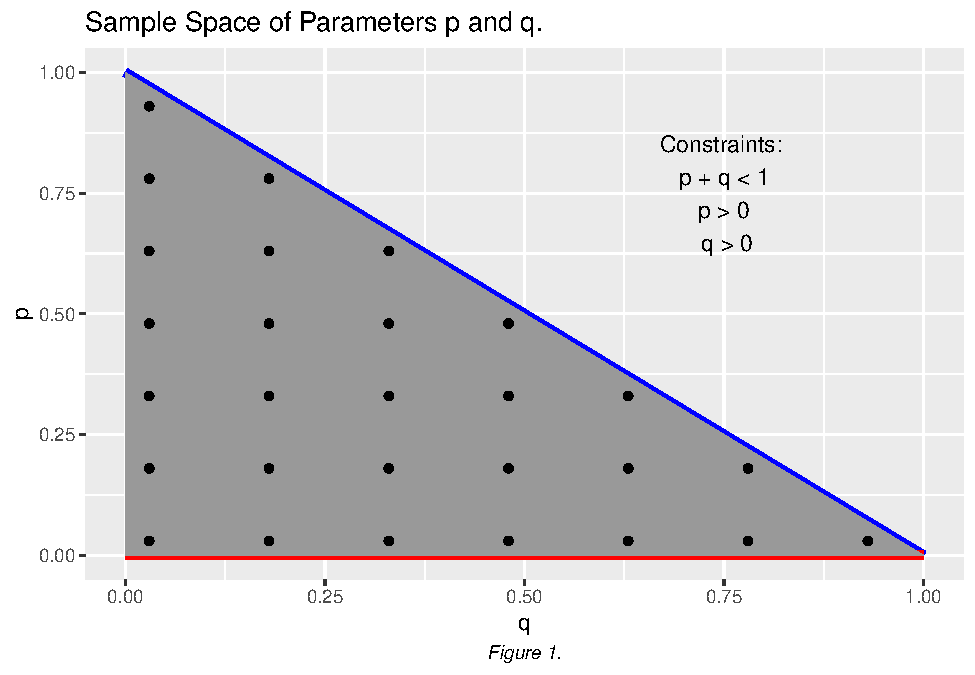
\includegraphics{Genetics_Faizan_HW1_v2_files/figure-latex/unnamed-chunk-1-1.pdf}

\subsection{Data}\label{data}

\begin{verbatim}
## Loading required package: knitr
\end{verbatim}

\begin{longtable}[]{@{}lrr@{}}
\caption{Table 1: Blood-Type and their counts in the sample
population.}\tabularnewline
\toprule
Blood-Type & Count & Frequency\tabularnewline
\midrule
\endfirsthead
\toprule
Blood-Type & Count & Frequency\tabularnewline
\midrule
\endhead
A & 9123 & 0.43\tabularnewline
B & 2987 & 0.14\tabularnewline
AB & 1269 & 0.06\tabularnewline
O & 7725 & 0.37\tabularnewline
Total & 21104 & 1.00\tabularnewline
\bottomrule
\end{longtable}

\section{Analysis and Results.}\label{analysis-and-results.}

\subsection{Newton-Raphson Algorithm}\label{newton-raphson-algorithm}

\begin{Shaded}
\begin{Highlighting}[]
\CommentTok{# The log likelihood function,}
\NormalTok{loglikf =}\StringTok{ }\ControlFlowTok{function}\NormalTok{(p, q) \{}

\NormalTok{  f =}\StringTok{ }\NormalTok{n_A }\OperatorTok{*}\StringTok{ }\KeywordTok{log}\NormalTok{(p}\OperatorTok{^}\DecValTok{2}\OperatorTok{+}\DecValTok{2}\OperatorTok{*}\NormalTok{p}\OperatorTok{*}\NormalTok{(}\DecValTok{1}\NormalTok{−p−q)) }\OperatorTok{+}\StringTok{ }\NormalTok{n_B}\OperatorTok{*}\KeywordTok{log}\NormalTok{(q}\OperatorTok{^}\DecValTok{2}\OperatorTok{+}\DecValTok{2}\OperatorTok{*}\NormalTok{q}\OperatorTok{*}\NormalTok{(}\DecValTok{1}\NormalTok{−p−q)) }\OperatorTok{+}\StringTok{ }\NormalTok{n_AB}\OperatorTok{*}\KeywordTok{log}\NormalTok{(}\DecValTok{2}\OperatorTok{*}\NormalTok{p}\OperatorTok{*}\NormalTok{q) }\OperatorTok{+}\StringTok{ }\NormalTok{n_O}\OperatorTok{*}\KeywordTok{log}\NormalTok{((}\DecValTok{1}\NormalTok{−p−q)}\OperatorTok{^}\DecValTok{2}\NormalTok{)}
  \KeywordTok{return}\NormalTok{(f)}
\NormalTok{\}}

\CommentTok{# Function that calculates the full first derivative. }
\NormalTok{Df =}\StringTok{ }\ControlFlowTok{function}\NormalTok{(p, q)\{}
  
\NormalTok{  dfp =}\StringTok{ }\NormalTok{(}\DecValTok{2}\OperatorTok{*}\NormalTok{n_B)}\OperatorTok{/}\NormalTok{(}\DecValTok{2}\OperatorTok{*}\NormalTok{p}\OperatorTok{+}\NormalTok{q}\OperatorTok{-}\DecValTok{2}\NormalTok{)}\OperatorTok{+}\NormalTok{n_A}\OperatorTok{*}\NormalTok{(}\DecValTok{1}\OperatorTok{/}\NormalTok{(p}\OperatorTok{+}\DecValTok{2}\OperatorTok{*}\NormalTok{q}\OperatorTok{-}\DecValTok{2}\NormalTok{)}\OperatorTok{+}\DecValTok{1}\OperatorTok{/}\NormalTok{p)}\OperatorTok{+}\NormalTok{n_AB}\OperatorTok{/}\NormalTok{p}\OperatorTok{-}\NormalTok{(}\DecValTok{2}\OperatorTok{*}\NormalTok{n_O)}\OperatorTok{/}\NormalTok{(}\OperatorTok{-}\NormalTok{p}\OperatorTok{-}\NormalTok{q}\OperatorTok{+}\DecValTok{1}\NormalTok{)}
  
\NormalTok{  dfq =}\StringTok{ }\NormalTok{(}\DecValTok{2}\OperatorTok{*}\NormalTok{n_A)}\OperatorTok{/}\NormalTok{(}\DecValTok{2}\OperatorTok{*}\NormalTok{q}\OperatorTok{+}\NormalTok{p}\OperatorTok{-}\DecValTok{2}\NormalTok{)}\OperatorTok{+}\NormalTok{n_B}\OperatorTok{*}\NormalTok{(}\DecValTok{1}\OperatorTok{/}\NormalTok{(q}\OperatorTok{+}\DecValTok{2}\OperatorTok{*}\NormalTok{p}\OperatorTok{-}\DecValTok{2}\NormalTok{)}\OperatorTok{+}\DecValTok{1}\OperatorTok{/}\NormalTok{q)}\OperatorTok{+}\NormalTok{n_AB}\OperatorTok{/}\NormalTok{q}\OperatorTok{-}\NormalTok{(}\DecValTok{2}\OperatorTok{*}\NormalTok{n_O)}\OperatorTok{/}\NormalTok{(}\OperatorTok{-}\NormalTok{q}\OperatorTok{-}\NormalTok{p}\OperatorTok{+}\DecValTok{1}\NormalTok{)}
  
  \KeywordTok{return}\NormalTok{( }\KeywordTok{c}\NormalTok{(dfp, dfq) )}
\NormalTok{\}}

\CommentTok{# Function that calculates the Hessian.}
\NormalTok{DDf =}\StringTok{ }\ControlFlowTok{function}\NormalTok{(p, q) \{}
  
\NormalTok{    d2fpp =}\StringTok{ }\OperatorTok{-}\NormalTok{(}\DecValTok{4}\OperatorTok{*}\NormalTok{n_B)}\OperatorTok{/}\NormalTok{(}\DecValTok{2}\OperatorTok{*}\NormalTok{p}\OperatorTok{+}\NormalTok{q}\OperatorTok{-}\DecValTok{2}\NormalTok{)}\OperatorTok{^}\DecValTok{2}\OperatorTok{+}\NormalTok{n_A}\OperatorTok{*}\NormalTok{(}\OperatorTok{-}\DecValTok{1}\OperatorTok{/}\NormalTok{(p}\OperatorTok{+}\DecValTok{2}\OperatorTok{*}\NormalTok{q}\OperatorTok{-}\DecValTok{2}\NormalTok{)}\OperatorTok{^}\DecValTok{2}\OperatorTok{-}\DecValTok{1}\OperatorTok{/}\NormalTok{p}\OperatorTok{^}\DecValTok{2}\NormalTok{)}\OperatorTok{-}\NormalTok{n_AB}\OperatorTok{/}\NormalTok{p}\OperatorTok{^}\DecValTok{2}\OperatorTok{-}\NormalTok{(}\DecValTok{2}\OperatorTok{*}\NormalTok{n_O)}\OperatorTok{/}\NormalTok{(}\OperatorTok{-}\NormalTok{p}\OperatorTok{-}\NormalTok{q}\OperatorTok{+}\DecValTok{1}\NormalTok{)}\OperatorTok{^}\DecValTok{2}
\NormalTok{    a =}\StringTok{ }\NormalTok{d2fpp}
\NormalTok{    d2fqp =}\StringTok{ }\OperatorTok{-}\NormalTok{(}\DecValTok{2}\OperatorTok{*}\NormalTok{n_A)}\OperatorTok{/}\NormalTok{(}\DecValTok{2}\OperatorTok{*}\NormalTok{q}\OperatorTok{+}\NormalTok{p}\OperatorTok{-}\DecValTok{2}\NormalTok{)}\OperatorTok{^}\DecValTok{2}\OperatorTok{-}\NormalTok{(}\DecValTok{2}\OperatorTok{*}\NormalTok{n_B)}\OperatorTok{/}\NormalTok{(q}\OperatorTok{+}\DecValTok{2}\OperatorTok{*}\NormalTok{p}\OperatorTok{-}\DecValTok{2}\NormalTok{)}\OperatorTok{^}\DecValTok{2}\OperatorTok{-}\NormalTok{(}\DecValTok{2}\OperatorTok{*}\NormalTok{n_O)}\OperatorTok{/}\NormalTok{(}\OperatorTok{-}\NormalTok{q}\OperatorTok{-}\NormalTok{p}\OperatorTok{+}\DecValTok{1}\NormalTok{)}\OperatorTok{^}\DecValTok{2}
\NormalTok{    c =}\StringTok{ }\NormalTok{d2fqp    }
\NormalTok{    d2fqq =}\StringTok{ }\OperatorTok{-}\NormalTok{(}\DecValTok{4}\OperatorTok{*}\NormalTok{n_A)}\OperatorTok{/}\NormalTok{(}\DecValTok{2}\OperatorTok{*}\NormalTok{q}\OperatorTok{+}\NormalTok{p}\OperatorTok{-}\DecValTok{2}\NormalTok{)}\OperatorTok{^}\DecValTok{2}\OperatorTok{+}\NormalTok{n_B}\OperatorTok{*}\NormalTok{(}\OperatorTok{-}\DecValTok{1}\OperatorTok{/}\NormalTok{(q}\OperatorTok{+}\DecValTok{2}\OperatorTok{*}\NormalTok{p}\OperatorTok{-}\DecValTok{2}\NormalTok{)}\OperatorTok{^}\DecValTok{2}\OperatorTok{-}\DecValTok{1}\OperatorTok{/}\NormalTok{q}\OperatorTok{^}\DecValTok{2}\NormalTok{)}\OperatorTok{-}\NormalTok{n_AB}\OperatorTok{/}\NormalTok{q}\OperatorTok{^}\DecValTok{2}\OperatorTok{-}\NormalTok{(}\DecValTok{2}\OperatorTok{*}\NormalTok{n_O)}\OperatorTok{/}\NormalTok{(}\OperatorTok{-}\NormalTok{q}\OperatorTok{-}\NormalTok{p}\OperatorTok{+}\DecValTok{1}\NormalTok{)}\OperatorTok{^}\DecValTok{2}
\NormalTok{    d =}\StringTok{ }\NormalTok{d2fqq}
\NormalTok{    d2fpq =}\StringTok{ }\OperatorTok{-}\NormalTok{(}\DecValTok{2}\OperatorTok{*}\NormalTok{n_B)}\OperatorTok{/}\NormalTok{(}\DecValTok{2}\OperatorTok{*}\NormalTok{p}\OperatorTok{+}\NormalTok{q}\OperatorTok{-}\DecValTok{2}\NormalTok{)}\OperatorTok{^}\DecValTok{2}\OperatorTok{-}\NormalTok{(}\DecValTok{2}\OperatorTok{*}\NormalTok{n_A)}\OperatorTok{/}\NormalTok{(p}\OperatorTok{+}\DecValTok{2}\OperatorTok{*}\NormalTok{q}\OperatorTok{-}\DecValTok{2}\NormalTok{)}\OperatorTok{^}\DecValTok{2}\OperatorTok{-}\NormalTok{(}\DecValTok{2}\OperatorTok{*}\NormalTok{n_O)}\OperatorTok{/}\NormalTok{(}\OperatorTok{-}\NormalTok{p}\OperatorTok{-}\NormalTok{q}\OperatorTok{+}\DecValTok{1}\NormalTok{)}\OperatorTok{^}\DecValTok{2}
\NormalTok{    b =}\StringTok{ }\NormalTok{d2fpq}
    
\NormalTok{    H =}\StringTok{ }\KeywordTok{matrix}\NormalTok{( }\KeywordTok{c}\NormalTok{(a, b, c, d), }\DataTypeTok{nrow =} \DecValTok{2}\NormalTok{)}
    \KeywordTok{return}\NormalTok{(H)}
\NormalTok{\}}
\end{Highlighting}
\end{Shaded}

\begin{Shaded}
\begin{Highlighting}[]
\NormalTok{nr_algo =}\StringTok{ }\ControlFlowTok{function}\NormalTok{(}\DataTypeTok{p0 =}\NormalTok{ .}\DecValTok{34}\NormalTok{,  }\DataTypeTok{q0 =}\NormalTok{ .}\DecValTok{34}\NormalTok{, }\DataTypeTok{maxiter =} \DecValTok{100}\NormalTok{, }\DataTypeTok{epsilon_p =}\NormalTok{ .}\DecValTok{000000001}\NormalTok{, }\DataTypeTok{epsilon_q =}\NormalTok{ .}\DecValTok{000000001}\NormalTok{)\{}

  \CommentTok{# p0 + q0 < 1 # contraint}
  
\NormalTok{  x0 =}\StringTok{ }\KeywordTok{c}\NormalTok{(p0, q0)}
\NormalTok{  x1  =}\StringTok{  }\NormalTok{x0  }\OperatorTok{-}\StringTok{  }\KeywordTok{solve}\NormalTok{(}\KeywordTok{DDf}\NormalTok{(x0[}\DecValTok{1}\NormalTok{], x0[}\DecValTok{2}\NormalTok{])) }\OperatorTok\StringTok{ }\KeywordTok{Df}\NormalTok{(x0[}\DecValTok{1}\NormalTok{], x0[}\DecValTok{2}\NormalTok{])}

\NormalTok{  p_NN =}\StringTok{  }\KeywordTok{c}\NormalTok{(x0[}\DecValTok{1}\NormalTok{], x1[}\DecValTok{1}\NormalTok{])}
\NormalTok{  q_NN =}\StringTok{  }\KeywordTok{c}\NormalTok{(x0[}\DecValTok{2}\NormalTok{], x1[}\DecValTok{2}\NormalTok{])}
  
\NormalTok{  j =}\StringTok{ }\DecValTok{2}
  \ControlFlowTok{while}\NormalTok{( }\OperatorTok{!}\NormalTok{( ( }\KeywordTok{abs}\NormalTok{(x1[}\DecValTok{1}\NormalTok{] }\OperatorTok{-}\StringTok{ }\NormalTok{x0[}\DecValTok{1}\NormalTok{]) }\OperatorTok{<}\StringTok{ }\NormalTok{epsilon_p }\OperatorTok{&}\StringTok{ }\KeywordTok{abs}\NormalTok{(x1[}\DecValTok{2}\NormalTok{] }\OperatorTok{-}\StringTok{ }\NormalTok{x0[}\DecValTok{2}\NormalTok{]) }\OperatorTok{<}\StringTok{ }\NormalTok{epsilon_q }\OperatorTok{|}\StringTok{ }\NormalTok{j }\OperatorTok{>}\StringTok{ }\NormalTok{maxiter ) ) ) \{}
  
\NormalTok{    x0 =}\StringTok{ }\NormalTok{x1}
  
\NormalTok{    x1  =}\StringTok{  }\NormalTok{x0  }\OperatorTok{-}\StringTok{  }\KeywordTok{solve}\NormalTok{(}\KeywordTok{DDf}\NormalTok{(x0[}\DecValTok{1}\NormalTok{], x0[}\DecValTok{2}\NormalTok{])) }\OperatorTok\StringTok{ }\KeywordTok{Df}\NormalTok{(x0[}\DecValTok{1}\NormalTok{], x0[}\DecValTok{2}\NormalTok{])}
  \CommentTok{# 2x1 =  2X1 -            2x2            %*%        2x1}
    
\NormalTok{    j =}\StringTok{ }\NormalTok{j }\OperatorTok{+}\StringTok{ }\DecValTok{1}
\NormalTok{    p_NN[j] =}\StringTok{  }\NormalTok{x1[}\DecValTok{1}\NormalTok{]}
\NormalTok{    q_NN[j] =}\StringTok{  }\NormalTok{x1[}\DecValTok{2}\NormalTok{]}
\NormalTok{  \}}
  
  \CommentTok{#j = j - 1}
\NormalTok{  results_data =}\StringTok{ }\KeywordTok{data.frame}\NormalTok{(}\DataTypeTok{p0 =}\NormalTok{ p0, }\DataTypeTok{q0 =}\NormalTok{ q0, }\DataTypeTok{maxiter =}\NormalTok{ maxiter, }\DataTypeTok{epsilon_p =}\NormalTok{ epsilon_p, }\DataTypeTok{epsilon_q =}\NormalTok{ epsilon_q, }\DataTypeTok{distance_p0q0_to_pq =}\NormalTok{ ((x1[}\DecValTok{1}\NormalTok{] }\OperatorTok{-}\StringTok{ }\NormalTok{p0)}\OperatorTok{^}\DecValTok{2} \OperatorTok{+}\NormalTok{(x1[}\DecValTok{2}\NormalTok{]}\OperatorTok{-}\NormalTok{q0)}\OperatorTok{^}\DecValTok{2}\NormalTok{)}\OperatorTok{^}\NormalTok{.}\DecValTok{5}\NormalTok{ , }\DataTypeTok{j =}\NormalTok{ j, }\DataTypeTok{p =}\NormalTok{ x1[}\DecValTok{1}\NormalTok{], }\DataTypeTok{q =}\NormalTok{ x1[}\DecValTok{2}\NormalTok{])}
  
\NormalTok{  p_q_data =}\StringTok{ }\KeywordTok{data.frame}\NormalTok{(}\DataTypeTok{j =} \DecValTok{1}\OperatorTok{:}\NormalTok{j, }\DataTypeTok{p_NN =}\NormalTok{ p_NN, }\DataTypeTok{q_NN =}\NormalTok{ q_NN)}
  
  \KeywordTok{return}\NormalTok{(}\KeywordTok{list}\NormalTok{( results_data, p_q_data))}
  \CommentTok{#return(list(results_data$results_data = results_data, p_q_data$p_q_data = p_q_data))}
\NormalTok{\}}

\KeywordTok{nr_algo}\NormalTok{()}
\end{Highlighting}
\end{Shaded}

\begin{verbatim}
## [[1]]
##     p0   q0 maxiter epsilon_p epsilon_q distance_p0q0_to_pq  j         p
## 1 0.34 0.34     100     1e-09     1e-09            0.239235 10 0.2876856
##          q
## 1 0.106555
## 
## [[2]]
##     j      p_NN       q_NN
## 1   1 0.3400000 0.34000000
## 2   2 0.4271137 0.02195062
## 3   3 0.2940355 0.03989035
## 4   4 0.3002998 0.06551315
## 5   5 0.2922187 0.09143553
## 6   6 0.2882774 0.10459457
## 7   7 0.2876952 0.10652301
## 8   8 0.2876856 0.10655499
## 9   9 0.2876856 0.10655500
## 10 10 0.2876856 0.10655500
\end{verbatim}

\begin{Shaded}
\begin{Highlighting}[]
\NormalTok{p0_vec =}\StringTok{ }\KeywordTok{rep}\NormalTok{(}\KeywordTok{rep}\NormalTok{(}\KeywordTok{seq}\NormalTok{(.}\DecValTok{01}\NormalTok{,.}\DecValTok{349}\NormalTok{, }\DataTypeTok{length.out =} \DecValTok{4}\NormalTok{ ), }\DecValTok{4}\NormalTok{), }\DecValTok{4}\NormalTok{)}
\NormalTok{q0_vec =}\StringTok{ }\KeywordTok{rep}\NormalTok{(}\KeywordTok{rep}\NormalTok{(}\KeywordTok{seq}\NormalTok{(.}\DecValTok{01}\NormalTok{,.}\DecValTok{349}\NormalTok{, }\DataTypeTok{length.out =} \DecValTok{4}\NormalTok{ ), }\DataTypeTok{each =} \DecValTok{4}\NormalTok{), }\DecValTok{4}\NormalTok{)}

\NormalTok{p0_vec =}\StringTok{ }\NormalTok{pi}
\NormalTok{q0_vec =}\StringTok{ }\NormalTok{qi}

\NormalTok{epsilon_p_vec =}\StringTok{ }\KeywordTok{rep}\NormalTok{(}\KeywordTok{c}\NormalTok{(}\DecValTok{10}\OperatorTok{^-}\DecValTok{3}\NormalTok{, }\DecValTok{10}\OperatorTok{^-}\DecValTok{5}\NormalTok{, }\DecValTok{10}\OperatorTok{^-}\DecValTok{10}\NormalTok{, }\DecValTok{10}\OperatorTok{^-}\DecValTok{15}\NormalTok{), }\DataTypeTok{each =} \KeywordTok{length}\NormalTok{(p0_vec))}
\NormalTok{epsilon_q_vec =}\StringTok{ }\KeywordTok{rep}\NormalTok{(}\KeywordTok{c}\NormalTok{(}\DecValTok{10}\OperatorTok{^-}\DecValTok{3}\NormalTok{, }\DecValTok{10}\OperatorTok{^-}\DecValTok{5}\NormalTok{, }\DecValTok{10}\OperatorTok{^-}\DecValTok{10}\NormalTok{, }\DecValTok{10}\OperatorTok{^-}\DecValTok{15}\NormalTok{), }\DataTypeTok{each =} \KeywordTok{length}\NormalTok{(p0_vec))}

\KeywordTok{sapply}\NormalTok{(}\KeywordTok{list}\NormalTok{(p0_vec, q0_vec, epsilon_p_vec, epsilon_q_vec), length )}
\end{Highlighting}
\end{Shaded}

\begin{verbatim}
## [1]  28  28 112 112
\end{verbatim}

\begin{Shaded}
\begin{Highlighting}[]
\NormalTok{combinations =}\StringTok{ }\KeywordTok{length}\NormalTok{(p0_vec)}

\NormalTok{nr_results =}\StringTok{ }\KeywordTok{data.frame}\NormalTok{()}
\NormalTok{nr_results_pq_vec =}\StringTok{ }\KeywordTok{data.frame}\NormalTok{()}
\NormalTok{t0_nr =}\StringTok{ }\KeywordTok{Sys.time}\NormalTok{()}
\ControlFlowTok{for}\NormalTok{ (i }\ControlFlowTok{in} \DecValTok{1}\OperatorTok{:}\NormalTok{combinations)\{}
  
\NormalTok{  results =}\StringTok{ }\KeywordTok{nr_algo}\NormalTok{(}\DataTypeTok{p0 =}\NormalTok{ p0_vec[i],  }
                    \DataTypeTok{q0 =}\NormalTok{ q0_vec[i], }
                    \DataTypeTok{maxiter =} \DecValTok{500}\NormalTok{, }
                    \DataTypeTok{epsilon_p =}\NormalTok{ epsilon_p_vec[i],}
                    \DataTypeTok{epsilon_q =}\NormalTok{ epsilon_q_vec[i])}
  
\NormalTok{  nr_results =}\StringTok{ }\KeywordTok{data.frame}\NormalTok{(}\KeywordTok{rbind}\NormalTok{(nr_results, results[[}\DecValTok{1}\NormalTok{]]))}
  \CommentTok{#nr_results_pq_vec[i,] = results[[2]]}
\NormalTok{\}}
\NormalTok{tf_nr =}\StringTok{ }\KeywordTok{Sys.time}\NormalTok{() }\OperatorTok{-}\StringTok{ }\NormalTok{t0_nr}
\NormalTok{tf_nr}
\end{Highlighting}
\end{Shaded}

\begin{verbatim}
## Time difference of 0.1009951 secs
\end{verbatim}

\begin{Shaded}
\begin{Highlighting}[]
\KeywordTok{dim}\NormalTok{(nr_results)}
\end{Highlighting}
\end{Shaded}

\begin{verbatim}
## [1] 28  9
\end{verbatim}

\begin{Shaded}
\begin{Highlighting}[]
\NormalTok{nr_results}
\end{Highlighting}
\end{Shaded}

\begin{verbatim}
##      p0   q0 maxiter epsilon_p epsilon_q distance_p0q0_to_pq   j
## 1  0.03 0.03     500     0.001     0.001        2.688169e-01   8
## 2  0.18 0.03     500     0.001     0.001        1.321241e-01   6
## 3  0.33 0.03     500     0.001     0.001        8.746998e-02   6
## 4  0.48 0.03     500     0.001     0.001        2.069911e-01   6
## 5  0.63 0.03     500     0.001     0.001        3.507701e-01   6
## 6  0.78 0.03     500     0.001     0.001        4.982310e-01   6
## 7  0.93 0.03     500     0.001     0.001        6.468604e-01   8
## 8  0.03 0.18     500     0.001     0.001        2.679478e-01   8
## 9  0.18 0.18     500     0.001     0.001        1.303476e-01   5
## 10 0.33 0.18     500     0.001     0.001        8.476396e-02   5
## 11 0.48 0.18     500     0.001     0.001        2.058616e-01   5
## 12 0.63 0.18     500     0.001     0.001        3.501058e-01   5
## 13 0.78 0.18     500     0.001     0.001        4.977627e-01   8
## 14 0.03 0.33     500     0.001     0.001        3.410711e-01   8
## 15 0.18 0.33     500     0.001     0.001       9.680478e+148 501
## 16 0.33 0.33     500     0.001     0.001        2.274185e-01   8
## 17 0.48 0.33     500     0.001     0.001        2.948093e-01   6
## 18 0.63 0.33     500     0.001     0.001        4.087870e-01   8
## 19 0.03 0.48     500     0.001     0.001        4.537213e-01   8
## 20 0.18 0.48     500     0.001     0.001        3.886618e-01   5
## 21 0.33 0.48     500     0.001     0.001        3.758347e-01   6
## 22 0.48 0.48     500     0.001     0.001        4.200548e-01   8
## 23 0.03 0.63     500     0.001     0.001        5.834351e-01   8
## 24 0.18 0.63     500     0.001     0.001        5.344070e-01  10
## 25 0.33 0.63     500     0.001     0.001        5.251525e-01   8
## 26 0.03 0.78     500     0.001     0.001        7.210617e-01   8
## 27 0.18 0.78     500     0.001     0.001        6.820006e-01   8
## 28 0.03 0.93     500     0.001     0.001        8.628298e-01   8
##                p              q
## 1   2.876856e-01   1.065550e-01
## 2   2.876858e-01   1.065542e-01
## 3   2.876859e-01   1.065540e-01
## 4   2.876858e-01   1.065542e-01
## 5   2.876857e-01   1.065546e-01
## 6   2.876856e-01   1.065550e-01
## 7   2.876857e-01   1.065547e-01
## 8   2.876856e-01   1.065550e-01
## 9   2.876858e-01   1.065543e-01
## 10  2.876862e-01   1.065530e-01
## 11  2.876856e-01   1.065550e-01
## 12  2.876848e-01   1.065535e-01
## 13  2.876856e-01   1.065550e-01
## 14  2.876856e-01   1.065550e-01
## 15 2.530074e+148 -9.344002e+148
## 16  2.876863e-01   1.065526e-01
## 17  2.876856e-01   1.065550e-01
## 18  2.876856e-01   1.065550e-01
## 19  2.876856e-01   1.065550e-01
## 20  2.876858e-01   1.065542e-01
## 21  2.876856e-01   1.065549e-01
## 22  2.876856e-01   1.065550e-01
## 23  2.876856e-01   1.065550e-01
## 24  2.876856e-01   1.065550e-01
## 25  2.876856e-01   1.065550e-01
## 26  2.876856e-01   1.065550e-01
## 27  2.876856e-01   1.065547e-01
## 28  2.876875e-01   1.065485e-01
\end{verbatim}

\subsection{EM Algorithm}\label{em-algorithm}

\begin{Shaded}
\begin{Highlighting}[]
\NormalTok{em_algo =}\StringTok{ }\ControlFlowTok{function}\NormalTok{( }\DataTypeTok{p0 =}\NormalTok{ .}\DecValTok{34}\NormalTok{,  }\DataTypeTok{q0 =}\NormalTok{ .}\DecValTok{34}\NormalTok{, }\DataTypeTok{maxiter =} \DecValTok{100}\NormalTok{, }\DataTypeTok{epsilon_p =}\NormalTok{ .}\DecValTok{00005}\NormalTok{,  }\DataTypeTok{epsilon_q =}\NormalTok{ .}\DecValTok{00005}\NormalTok{)\{}

      \CommentTok{# Starting estimates}
\NormalTok{      p_initial =}\StringTok{ }\NormalTok{p0}
\NormalTok{      q_initial =}\StringTok{ }\NormalTok{q0}
      
      \CommentTok{# Expectation Step}
                
\NormalTok{      E_nAA =}\StringTok{ }\NormalTok{n_A }\OperatorTok{*}\StringTok{ }\NormalTok{( (p0}\OperatorTok{^}\DecValTok{2}\NormalTok{) }\OperatorTok{/}\StringTok{ }\NormalTok{( p0}\OperatorTok{^}\DecValTok{2} \OperatorTok{+}\StringTok{ }\DecValTok{2}\OperatorTok{*}\NormalTok{p0}\OperatorTok{*}\NormalTok{(}\DecValTok{1}\OperatorTok{-}\NormalTok{p0}\OperatorTok{-}\NormalTok{q0) ) )}
\NormalTok{      E_nAO =}\StringTok{ }\NormalTok{n_A }\OperatorTok{*}\StringTok{ }\NormalTok{( (}\DecValTok{2}\OperatorTok{*}\NormalTok{p0}\OperatorTok{*}\NormalTok{(}\DecValTok{1}\OperatorTok{-}\NormalTok{p0}\OperatorTok{-}\NormalTok{q0)) }\OperatorTok{/}\StringTok{ }\NormalTok{( p0}\OperatorTok{^}\DecValTok{2} \OperatorTok{+}\StringTok{ }\DecValTok{2}\OperatorTok{*}\NormalTok{p0}\OperatorTok{*}\NormalTok{(}\DecValTok{1}\OperatorTok{-}\NormalTok{p0}\OperatorTok{-}\NormalTok{q0) ) )}
\NormalTok{      E_nBB =}\StringTok{ }\NormalTok{n_B }\OperatorTok{*}\StringTok{ }\NormalTok{( (q0}\OperatorTok{^}\DecValTok{2}\NormalTok{) }\OperatorTok{/}\StringTok{ }\NormalTok{( p0}\OperatorTok{^}\DecValTok{2} \OperatorTok{+}\StringTok{ }\DecValTok{2}\OperatorTok{*}\NormalTok{q0}\OperatorTok{*}\NormalTok{(}\DecValTok{1}\OperatorTok{-}\NormalTok{p0}\OperatorTok{-}\NormalTok{q0) ) )}
\NormalTok{      E_nBO =}\StringTok{ }\NormalTok{n_B }\OperatorTok{*}\StringTok{ }\NormalTok{( (}\DecValTok{2}\OperatorTok{*}\NormalTok{q0}\OperatorTok{*}\NormalTok{(}\DecValTok{1}\OperatorTok{-}\NormalTok{p0}\OperatorTok{-}\NormalTok{q0)) }\OperatorTok{/}\StringTok{ }\NormalTok{( q0}\OperatorTok{^}\DecValTok{2} \OperatorTok{+}\StringTok{ }\DecValTok{2}\OperatorTok{*}\NormalTok{p0}\OperatorTok{*}\NormalTok{(}\DecValTok{1}\OperatorTok{-}\NormalTok{p0}\OperatorTok{-}\NormalTok{q0) ) )}
      
      \CommentTok{# Maximization step}
      
\NormalTok{      p1 =}\StringTok{ }\NormalTok{(}\DecValTok{2}\OperatorTok{*}\StringTok{ }\NormalTok{E_nAA }\OperatorTok{+}\StringTok{ }\NormalTok{E_nAO }\OperatorTok{+}\StringTok{ }\NormalTok{n_AB) }\OperatorTok{/}\StringTok{ }\NormalTok{(}\DecValTok{2}\OperatorTok{*}\NormalTok{n)}
\NormalTok{      q1 =}\StringTok{ }\NormalTok{(}\DecValTok{2}\OperatorTok{*}\StringTok{ }\NormalTok{E_nBB }\OperatorTok{+}\StringTok{ }\NormalTok{E_nBO }\OperatorTok{+}\StringTok{ }\NormalTok{n_AB) }\OperatorTok{/}\StringTok{ }\NormalTok{(}\DecValTok{2}\OperatorTok{*}\NormalTok{n)}
      
      
\NormalTok{      p_NN =}\StringTok{ }\KeywordTok{c}\NormalTok{(p0, p1)}
\NormalTok{      q_NN =}\StringTok{ }\KeywordTok{c}\NormalTok{(q0, q1)}
      
      \CommentTok{# 2 assumptions: hwe and }
\NormalTok{      j =}\StringTok{ }\DecValTok{2}
      \ControlFlowTok{while}\NormalTok{( }\OperatorTok{!}\NormalTok{( }\KeywordTok{abs}\NormalTok{(p1 }\OperatorTok{-}\StringTok{ }\NormalTok{p0) }\OperatorTok{<}\StringTok{ }\NormalTok{epsilon_p }\OperatorTok{&}\StringTok{ }\KeywordTok{abs}\NormalTok{(q1 }\OperatorTok{-}\StringTok{ }\NormalTok{q0) }\OperatorTok{<}\StringTok{ }\NormalTok{epsilon_q }\OperatorTok{|}\StringTok{ }\NormalTok{j }\OperatorTok{>}\StringTok{ }\NormalTok{maxiter) ) \{ }
        
\NormalTok{              p0 =}\StringTok{ }\NormalTok{p1}
\NormalTok{              q0 =}\StringTok{ }\NormalTok{q1}
        
              \CommentTok{# Expectation Step}
            
\NormalTok{              E_nAA =}\StringTok{ }\NormalTok{n_A }\OperatorTok{*}\StringTok{ }\NormalTok{( (p0}\OperatorTok{^}\DecValTok{2}\NormalTok{) }\OperatorTok{/}\StringTok{ }\NormalTok{( p0}\OperatorTok{^}\DecValTok{2} \OperatorTok{+}\StringTok{ }\DecValTok{2}\OperatorTok{*}\NormalTok{p0}\OperatorTok{*}\NormalTok{(}\DecValTok{1}\OperatorTok{-}\NormalTok{p0}\OperatorTok{-}\NormalTok{q0) ) )}
\NormalTok{              E_nAO =}\StringTok{ }\NormalTok{n_A }\OperatorTok{*}\StringTok{ }\NormalTok{( (}\DecValTok{2}\OperatorTok{*}\NormalTok{p0}\OperatorTok{*}\NormalTok{(}\DecValTok{1}\OperatorTok{-}\NormalTok{p0}\OperatorTok{-}\NormalTok{q0)) }\OperatorTok{/}\StringTok{ }\NormalTok{( p0}\OperatorTok{^}\DecValTok{2} \OperatorTok{+}\StringTok{ }\DecValTok{2}\OperatorTok{*}\NormalTok{p0}\OperatorTok{*}\NormalTok{(}\DecValTok{1}\OperatorTok{-}\NormalTok{p0}\OperatorTok{-}\NormalTok{q0) ) )}
\NormalTok{              E_nBB =}\StringTok{ }\NormalTok{n_B }\OperatorTok{*}\StringTok{ }\NormalTok{( (q0}\OperatorTok{^}\DecValTok{2}\NormalTok{) }\OperatorTok{/}\StringTok{ }\NormalTok{( q0}\OperatorTok{^}\DecValTok{2} \OperatorTok{+}\StringTok{ }\DecValTok{2}\OperatorTok{*}\NormalTok{q0}\OperatorTok{*}\NormalTok{(}\DecValTok{1}\OperatorTok{-}\NormalTok{p0}\OperatorTok{-}\NormalTok{q0) ) )}
\NormalTok{              E_nBO =}\StringTok{ }\NormalTok{n_B }\OperatorTok{*}\StringTok{ }\NormalTok{( (}\DecValTok{2}\OperatorTok{*}\NormalTok{q0}\OperatorTok{*}\NormalTok{(}\DecValTok{1}\OperatorTok{-}\NormalTok{p0}\OperatorTok{-}\NormalTok{q0)) }\OperatorTok{/}\StringTok{ }\NormalTok{( q0}\OperatorTok{^}\DecValTok{2} \OperatorTok{+}\StringTok{ }\DecValTok{2}\OperatorTok{*}\NormalTok{q0}\OperatorTok{*}\NormalTok{(}\DecValTok{1}\OperatorTok{-}\NormalTok{p0}\OperatorTok{-}\NormalTok{q0) ) )}
              
              \CommentTok{# Maximization step}
              
\NormalTok{              p1 =}\StringTok{ }\NormalTok{(}\DecValTok{2}\OperatorTok{*}\StringTok{ }\NormalTok{E_nAA }\OperatorTok{+}\StringTok{ }\NormalTok{E_nAO }\OperatorTok{+}\StringTok{ }\NormalTok{n_AB) }\OperatorTok{/}\StringTok{ }\NormalTok{(}\DecValTok{2}\OperatorTok{*}\NormalTok{n) }
\NormalTok{              q1 =}\StringTok{ }\NormalTok{(}\DecValTok{2}\OperatorTok{*}\StringTok{ }\NormalTok{E_nBB }\OperatorTok{+}\StringTok{ }\NormalTok{E_nBO }\OperatorTok{+}\StringTok{ }\NormalTok{n_AB) }\OperatorTok{/}\StringTok{ }\NormalTok{(}\DecValTok{2}\OperatorTok{*}\NormalTok{n)}
              
\NormalTok{              j =}\StringTok{ }\NormalTok{j }\OperatorTok{+}\StringTok{ }\DecValTok{1}
\NormalTok{              p_NN[j] =}\StringTok{ }\NormalTok{p1}
\NormalTok{              q_NN[j] =}\StringTok{ }\NormalTok{q1}
\NormalTok{      \}}
      
\NormalTok{      results_data =}\StringTok{ }\KeywordTok{data.frame}\NormalTok{(}\DataTypeTok{p0 =}\NormalTok{ p_initial, }\DataTypeTok{q0 =}\NormalTok{ q_initial, }\DataTypeTok{maxiter =}\NormalTok{ maxiter, }\DataTypeTok{epsilon_p =}\NormalTok{ epsilon_p, }\DataTypeTok{epsilon_q =}\NormalTok{ epsilon_q, }\DataTypeTok{distance_p0q0_to_pq =}\NormalTok{ ((p1 }\OperatorTok{-}\StringTok{ }\NormalTok{p_initial)}\OperatorTok{^}\DecValTok{2} \OperatorTok{+}\NormalTok{(q1}\OperatorTok{-}\NormalTok{q_initial)}\OperatorTok{^}\DecValTok{2}\NormalTok{)}\OperatorTok{^}\NormalTok{.}\DecValTok{5}\NormalTok{ , }\DataTypeTok{j =}\NormalTok{ j, }\DataTypeTok{p =}\NormalTok{ p1, }\DataTypeTok{q =}\NormalTok{ q1)}
  
\NormalTok{      p_q_data =}\StringTok{ }\KeywordTok{data.frame}\NormalTok{(}\DataTypeTok{j =} \DecValTok{1}\OperatorTok{:}\NormalTok{j, }\DataTypeTok{p_NN =}\NormalTok{ p_NN, }\DataTypeTok{q_NN =}\NormalTok{ q_NN)}
  
      \KeywordTok{return}\NormalTok{(}\KeywordTok{list}\NormalTok{( results_data, p_q_data))}

\NormalTok{\}}

\CommentTok{#em_algo()}
\end{Highlighting}
\end{Shaded}

\begin{Shaded}
\begin{Highlighting}[]
\CommentTok{# p0_vec = rep(rep(seq(.01,.349, length.out = 4 ), 4), 4)}
\CommentTok{# q0_vec = rep(rep(seq(.01,.349, length.out = 4 ), each = 4), 4)}

\NormalTok{p0_vec =}\StringTok{ }\NormalTok{pi}
\NormalTok{q0_vec =}\StringTok{ }\NormalTok{qi}

\CommentTok{# epsilon_p_vec = rep(c(10^-3, 10^-5, 10^-10, 10^-15), each = 16)}
\CommentTok{# epsilon_q_vec = rep(c(10^-3, 10^-5, 10^-10, 10^-15), each = 16)}


\NormalTok{epsilon_p_vec =}\StringTok{ }\KeywordTok{rep}\NormalTok{(}\KeywordTok{c}\NormalTok{(}\DecValTok{10}\OperatorTok{^-}\DecValTok{3}\NormalTok{, }\DecValTok{10}\OperatorTok{^-}\DecValTok{5}\NormalTok{, }\DecValTok{10}\OperatorTok{^-}\DecValTok{10}\NormalTok{, }\DecValTok{10}\OperatorTok{^-}\DecValTok{15}\NormalTok{), }\DataTypeTok{each =} \KeywordTok{length}\NormalTok{(p0_vec))}
\NormalTok{epsilon_q_vec =}\StringTok{ }\KeywordTok{rep}\NormalTok{(}\KeywordTok{c}\NormalTok{(}\DecValTok{10}\OperatorTok{^-}\DecValTok{3}\NormalTok{, }\DecValTok{10}\OperatorTok{^-}\DecValTok{5}\NormalTok{, }\DecValTok{10}\OperatorTok{^-}\DecValTok{10}\NormalTok{, }\DecValTok{10}\OperatorTok{^-}\DecValTok{15}\NormalTok{), }\DataTypeTok{each =} \KeywordTok{length}\NormalTok{(p0_vec))}

\KeywordTok{sapply}\NormalTok{(}\KeywordTok{list}\NormalTok{(p0_vec, q0_vec, epsilon_p_vec, epsilon_q_vec), length )}
\end{Highlighting}
\end{Shaded}

\begin{verbatim}
## [1]  28  28 112 112
\end{verbatim}

\begin{Shaded}
\begin{Highlighting}[]
\NormalTok{combinations =}\StringTok{ }\KeywordTok{length}\NormalTok{(p0_vec)}

\NormalTok{em_results =}\StringTok{ }\KeywordTok{data.frame}\NormalTok{()}
\NormalTok{em_results_pq_vec =}\StringTok{ }\KeywordTok{data.frame}\NormalTok{()}

\NormalTok{t0_em =}\StringTok{ }\KeywordTok{Sys.time}\NormalTok{()}
\ControlFlowTok{for}\NormalTok{ (i }\ControlFlowTok{in} \DecValTok{1}\OperatorTok{:}\NormalTok{combinations)\{}
  
\NormalTok{  results =}\StringTok{ }\KeywordTok{em_algo}\NormalTok{(}\DataTypeTok{p0 =}\NormalTok{ p0_vec[i],  }
                    \DataTypeTok{q0 =}\NormalTok{ q0_vec[i], }
                    \DataTypeTok{maxiter =} \DecValTok{100}\NormalTok{, }
                    \DataTypeTok{epsilon_p =}\NormalTok{ epsilon_p_vec[i],}
                    \DataTypeTok{epsilon_q =}\NormalTok{ epsilon_q_vec[i])}
  
\NormalTok{  em_results =}\StringTok{ }\KeywordTok{rbind}\NormalTok{(em_results, results[[}\DecValTok{1}\NormalTok{]])}
  \CommentTok{#nr_results_pq_vec[i,] = results[[2]]}
\NormalTok{\}}
\NormalTok{tf_em =}\StringTok{ }\KeywordTok{Sys.time}\NormalTok{() }\OperatorTok{-}\StringTok{ }\NormalTok{t0_em}
\NormalTok{tf_em}
\end{Highlighting}
\end{Shaded}

\begin{verbatim}
## Time difference of 0.193994 secs
\end{verbatim}

\begin{Shaded}
\begin{Highlighting}[]
\KeywordTok{dim}\NormalTok{(em_results)}
\end{Highlighting}
\end{Shaded}

\begin{verbatim}
## [1] 28  9
\end{verbatim}

\begin{Shaded}
\begin{Highlighting}[]
\NormalTok{em_results}
\end{Highlighting}
\end{Shaded}

\begin{verbatim}
##      p0   q0 maxiter epsilon_p epsilon_q distance_p0q0_to_pq j         p
## 1  0.03 0.03     100     0.001     0.001          0.26861730 5 0.2874819
## 2  0.18 0.03     100     0.001     0.001          0.13208905 6 0.2876447
## 3  0.33 0.03     100     0.001     0.001          0.08752050 5 0.2875462
## 4  0.48 0.03     100     0.001     0.001          0.20700334 5 0.2876678
## 5  0.63 0.03     100     0.001     0.001          0.35063158 5 0.2878273
## 6  0.78 0.03     100     0.001     0.001          0.49817051 6 0.2877474
## 7  0.93 0.03     100     0.001     0.001          0.64674749 6 0.2878003
## 8  0.03 0.18     100     0.001     0.001          0.26800217 6 0.2877439
## 9  0.18 0.18     100     0.001     0.001          0.13029147 5 0.2876152
## 10 0.33 0.18     100     0.001     0.001          0.08476216 5 0.2876925
## 11 0.48 0.18     100     0.001     0.001          0.20571642 5 0.2878393
## 12 0.63 0.18     100     0.001     0.001          0.35004019 6 0.2877507
## 13 0.78 0.18     100     0.001     0.001          0.49764083 6 0.2878075
## 14 0.03 0.33     100     0.001     0.001          0.34121546 5 0.2879157
## 15 0.18 0.33     100     0.001     0.001          0.24806050 5 0.2877601
## 16 0.33 0.33     100     0.001     0.001          0.22736067 5 0.2878912
## 17 0.48 0.33     100     0.001     0.001          0.29475484 6 0.2877625
## 18 0.63 0.33     100     0.001     0.001          0.40866598 6 0.2878237
## 19 0.03 0.48     100     0.001     0.001          0.45376189 5 0.2877985
## 20 0.18 0.48     100     0.001     0.001          0.38866903 6 0.2877280
## 21 0.33 0.48     100     0.001     0.001          0.37581515 6 0.2877868
## 22 0.48 0.48     100     0.001     0.001          0.41995078 6 0.2878832
## 23 0.03 0.63     100     0.001     0.001          0.58347148 5 0.2878337
## 24 0.18 0.63     100     0.001     0.001          0.53442216 6 0.2878159
## 25 0.33 0.63     100     0.001     0.001          0.52513845 7 0.2877753
## 26 0.03 0.78     100     0.001     0.001          0.72109246 6 0.2878003
## 27 0.18 0.78     100     0.001     0.001          0.68199664 8 0.2876443
## 28 0.03 0.93     100     0.001     0.001          0.86278901 7 0.2875268
##            q
## 1  0.1065398
## 2  0.1065515
## 3  0.1065344
## 4  0.1065422
## 5  0.1065528
## 6  0.1065588
## 7  0.1065626
## 8  0.1065611
## 9  0.1065505
## 10 0.1065514
## 11 0.1065593
## 12 0.1065593
## 13 0.1065633
## 14 0.1066002
## 15 0.1065682
## 16 0.1065728
## 17 0.1065606
## 18 0.1065648
## 19 0.1065836
## 20 0.1065589
## 21 0.1065632
## 22 0.1065702
## 23 0.1065874
## 24 0.1065664
## 25 0.1065619
## 26 0.1065660
## 27 0.1065521
## 28 0.1065409
\end{verbatim}

\section{Discussion}\label{discussion}

\subsection{Comparing Algorithm Speed and
Efficiency.}\label{comparing-algorithm-speed-and-efficiency.}

\subsection{Comparing Algorithms' robustness to initial
vaules.}\label{comparing-algorithms-robustness-to-initial-vaules.}

The sample space of the paramters is p, q \textgreater{} 0 and p + q
\textless{} 1. However, we need to be away from the boundry of the
sample space since near or at the boundry of the sample space the
Hessian Matrix can become sigular. To see the robustness to initial
values of the two algorithms we start from different initial values. We
choose these values such that one point is taken from each region and
the sample space is covered.

\subsection{Choosing the threshold for the stopping
criteria.}\label{choosing-the-threshold-for-the-stopping-criteria.}

The threshold can also be thought of as the accuracy we are fine with
the estimates.

First observation concerning the choice of threshold values is that the
smaller we make this, (the higher the accuray we demand), the more
iterations the algorithms take to reach as is expected.

In terms of how small the threshold should be and how much accuracy
should be demanded, is a trade between number of iterations and
computational cost versus accuracy of estimate.

In partical terms, we would never need an accuracy of greater than 5
decimal points when estimating the allele frequency in the population.
Similary, the minimum accuracy we would need would be at least 3 decimal
points, anything less would not be a very stable estimate. The number of
iterations increases by \ldots{} from an accuracy of 3 decimal points to
5 decimal points.

We can also see that the

\subsection{Computational Time.}\label{computational-time.}

In terms of computational time tf\_nr was faster by 92.1\%

\subsection{Choosing stopping
criteria.}\label{choosing-stopping-criteria.}

For the stopping criteria for the implementation of the two algorthims
we took the difference in absolute value between sequent estimates. The
distance measured in absolute values is called manhatten distance.
However, we could also look if the euclidian distance (L1, or L2) is
used instead. We know that euclidian distance is less than or equal to
manhattan distance.

However, this is not the most robust stopping criteria, because it is
possible that the subsequent change in estimates happens to be smaller
than the indicated threshold. One way to . Another thing that can
improve the robustness of the stopping criteria is to see check if the
rate of

Another thing that could improve the robustness is that instead of
looking at only two sequential estimates, to look at several sequential
estimates and

Another, thind to keep in mind is that, in several algorithms, there is
some randomness in built in the process. Hence, a stopping criteria that
is based on several sequential points of estimates and calculating two
averages and see if the decrease is small enough. This would be more
stable, since two sequential point estimates can be very close randomly,
but the genenral trend of the estimate points decrease is not small
enough for a given threshold or accuracy. Hence, it is a more robust
stopping criteria to look at a set of sequential points and comparing if
the average decrease between the two sets of sequential points is less
than a given threshold.

\subsection{Advantages and Disadvantages of the two
Algorithms.}\label{advantages-and-disadvantages-of-the-two-algorithms.}

\subsubsection{Advantages of Expectation Maximization
Algorithm}\label{advantages-of-expectation-maximization-algorithm}

\subsubsection{Disadvantage of Expectation Maximization
Algorithm}\label{disadvantage-of-expectation-maximization-algorithm}

\subsubsection{Advantages of Newton Raphson
Algorithm}\label{advantages-of-newton-raphson-algorithm}

\subsubsection{Disadvantage of Newton Raphson
Algorithm.}\label{disadvantage-of-newton-raphson-algorithm.}

One disadvantage in both algorithms is that it is possible that the
algorithm converges to a local instead of global minimum or maximum.

One way to determine if we have converged to a global maximum is to do a
dense search of the sample space and plot the graph of the
log-likelihood. This will

\subsection{}\label{section}

\section{References}\label{references}


\end{document}
